\chapter{Fundamentals}
\label{ch:Fundamentals}


%%%%%%%%%%%%%%%%%%%%%%%%%%%%%%%%%%%%%%%%%%%%%%%%%%%%%%%%%%%%%%%%%%%%%%%%%%%%%%%
                      %%Valve%%
%%%%%%%%%%%%%%%%%%%%%%%%%%%%%%%%%%%%%%%%%%%%%%%%%%%%%%%%%%%%%%%%%%%%%%%%%%%%%%%
\section{valve}
\label{sec:valve}

\subsection{Introduction of valve}
\label{sec:IntroductionOfValve}

The valve, a device made of closed sections, controls the pipeline fluid transport system. 
It is used to regulate the cross section of the pathway and the flow direction of the medium, 
with functions including inflow, shutoff, throttle, check, diversion, and overflow pressure relief, 
which is shown in the figure \ref{fig:ValveType}.\\

Valves for fluid control, ranging from basic globe valves to the most complex valves in automation control systems.
It can be utilized to regulate the flow of numerous types of fluids, including water, steam, oil, gas, slurry, various corrosive media, and liquid metals, among others.
The valve's working pressure ranges from 0.0013MPa to 1000MPa of ultra-high pressure, 
and its working temperature ranges from c-270°C of ultra-low temperature to 1430°C of high temperature. \cite{Valvebaidu}

\begin{figure}[htbp]
    \centering
    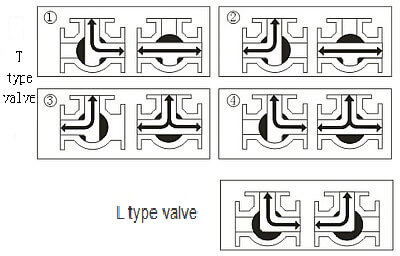
\includegraphics[width=0.3\textwidth]{figures/Fundamentals/TLtype.jpg}
    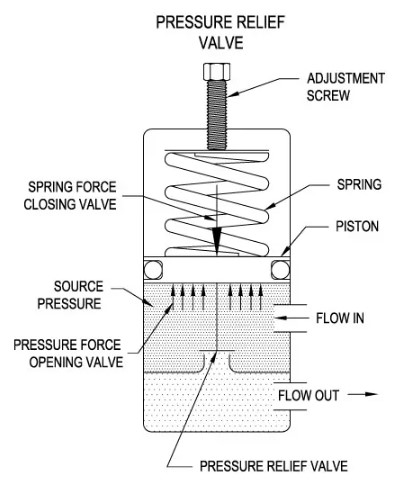
\includegraphics[width=0.3\textwidth]{figures/Fundamentals/PRelief.jpg}
    \caption{left:T and L type of valves \cite{TLtype}; right:Pressure Relief Valves \cite{PRvalve} }
    \label{fig:ValveType}
\end{figure}

A variety of transmission techniques, including manual, electric, hydraulic, pneumatic, 
electromagnetic movement, etc., can be used to control the valve. The valve can rely on the 
transmission device to perform lifting, sliding, rotating, and other actions under the influence of pressure, 
temperature, or other types of sensing signals to change the size of its flow channel area and carry out 
its control function.


%%%%%%%%%%%%%%%%%%%%%%%%%%%%%%%%%%%%%%%%%%%%%%%%%%%%%%%%%%%%%%%%%%%%%%%%%%%%%%%
\subsection{Principle of Globe Valve}
\label{sec:PrincipleofGlobeValve}

Based on their function, valves can be classified as shut-off valves, control valves, 
check valves, diverter valves, and safety valves, among others.\\

The most common valve is the shut-off valve. It contains globe valves, gate valves, 
ball valves and butterfly valves, etc. The low-friction force between the sealing surfaces 
during the opening and closing process is the main reason why valves are mostly utilized to 
obstruct fluid paths. Therefore, relatively resilient, and simple to produce.\\

A globe valve, as shown in the figure \ref*{fig:discs}, closes in a linear motion. This indicates that the closing member, 
which is referred to as a disc, slides vertically on and off the valve seat. Depending on how far the disc travels, 
the valve seat's opening changes. The regulation of a flow is suitable for such proportional variation. 
Following figure shows three basic disc of globe valves.\\

\begin{figure}[htbp]
    \centering
    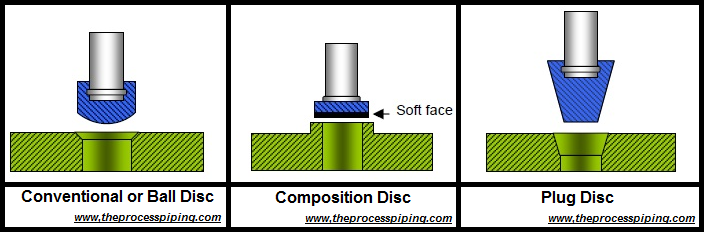
\includegraphics[width=0.7\textwidth]{Fundamentals/Globe-Valve-Discs.png}
    \caption{Different types of Globe-Valve-Discs \cite{discs}}
    \label{fig:discs}
\end{figure}

\begin{itemize}
    \item Conventional Disc or Ball Disc: Its primary function is to stop and start the flow. This valve is typically wide open or entirely closed and regulates the flow rarely.
    \item Composition Disc: Due to their resistant to erosion and can be closed without destroying the valve, composition discs are generally utilized in steam and hot water applications.
    \item Plug Type Disc: Because of its expansive seating area, the plug shutdown valve is the most effective of the three types for throttling. This surface is resistant to foreign objects and obstructions, and when the valve is wide open, it allows for maximum flow.
\end{itemize}

\begin{figure}[htbp]
    \centering
    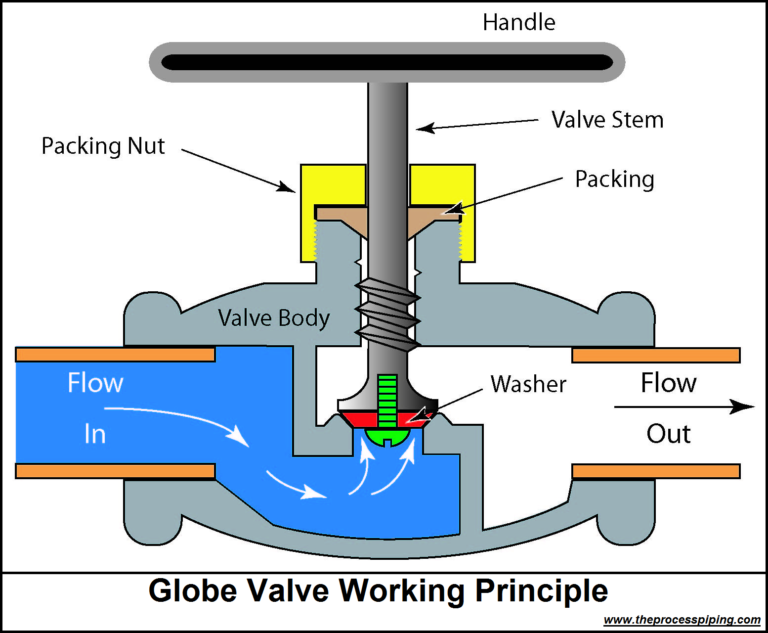
\includegraphics[width=0.5\textwidth]{Fundamentals/globe-valve-768x633.png}
    \caption{Working principle of globe valve \cite{WPfigure}}
    \label{fig:WP}
\end{figure}

The closing principle of the globe valve, as the sketch in figure \Ref*{fig:WP}, is that the stem of the globe valve applies pressure on the 
valve disc in the axial direction via applying torque to the stem, causing the valve disc's sealing 
surface to fit closely against the valve seat's sealing surface and preventing medium leakage along 
the gap between the sealing surfaces. The flow direction of the globe valve is always from top to bottom, 
indicating that the installation has a directionality \cite{WP}.\\

Compared to the other regularly used shut-off valve in industrial production. 
The globe control valve is structurally simpler and easier to manufacture and maintain than its predecessor. 
In regard to service life, the sealing surface of the globe valve is not easily worn or scratched, 
and there is no relative sliding between the valve disc and the sealing surface of the seat during 
the opening and shutting of the valve. As a result, there is minimal wear and scratching on the sealing surface, 
which increases the service life of the seal.


%%%%%%%%%%%%%%%%%%%%%%%%%%%%%%%%%%%%%%%%%%%%%%%%%%%%%%%%%%%%%%%%%%%%%%%%%%%%%%%
\subsection{Leakage and sealing of globe valves}
\label{sec:LeakageandSealingofglobevalves}

The sealing surface of the valve is the contact area between the valve disc and the valve seat. 
Primarily, its sealing is accomplished by compressing these two smooth sealing surfaces to prevent 
the medium from passing through the leakage channel. Leakage can occur for a number of causes, 
but the two main ones are gaps between the sealing surfaces and pressure on the sealing surfaces.\\

Different roughnesses of the valve's surfaces are the principal cause of the space between the sealing surfaces. 
Ideally, the space between the sealing surfaces should be smaller than the diameter of the fluid molecules. 
Even if the surface of the valve is highly polished, its roughness does not meet expectations. 
The pressure differential between the fluid pressure and the force applied to the component induces elastic or plastic 
deformation of the valve seat, which fills the irregularities on the sealing surface to prevent fluid leakage \cite{LeckagenPrinciple}.\\

The quality and structure of the disc and seat of the valve will influence the sealing performance. 
The quality is mostly decided by the selection of materials and the precision of manufacturing. 
Regarding the selection of materials, those with a low coefficient of friction, high elasticity, 
and resistance to corrosion should be used. This can improve the seal between the valve and seat, 
thus reducing leakage \cite{causedLeakage}.


%%%%%%%%%%%%%%%%%%%%%%%%%%%%%%%%%%%%%%%%%%%%%%%%%%%%%%%%%%%%%%%%%%%%%%%%%%%%%%%
                      %%Sensor%%
%%%%%%%%%%%%%%%%%%%%%%%%%%%%%%%%%%%%%%%%%%%%%%%%%%%%%%%%%%%%%%%%%%%%%%%%%%%%%%%
\section{Piezoelectric sensor}
\label{sec:PiezoelectricSensor}

\subsection{Introduction of Piezoelectric sensor}
\label{sec:IntroductionOfPiezoelectricSensor}
A sensor based on the piezoelectric effect is known as a piezoelectric sensor. When a force is applied to a piezoelectric material, 
an electrical charge is generated on its surface. This charge is converted by a charge amplifier into an electrical output, 
which is proportional to the external force. The element of the pressure sensor is sensitive to force, 
therefore it could measure physical quantities, such as force, pressure, acceleration, and vibration.\\

A piezoelectric sensor offers a broad frequency range, great sensitivity, a good signal-to-noise ratio, a simple design, and is lightweight. 
It can also measure various dynamic forces, mechanical vibrations, and shocks, which are used mostly in mechanics, acoustics, 
medicine, space exploration, etc. Certain piezoelectric materials have a low output DC response, 
requiring the application of a charge amplifier to overcome this disadvantage \cite{steinem2007}.


%%%%%%%%%%%%%%%%%%%%%%%%%%%%%%%%%%%%%%%%%%%%%%%%%%%%%%%%%%%%%%%%%%%%%%%%%%%%%%%
\subsection{Piezoelectric effect}
\label{sec:PiezoelectricEffect}
Positive and inverse piezoelectric effects are two subtypes of the piezoelectric effect. 
The positive piezoelectric effect, shown in the figure \Ref*{fig:PiezoEffect}, indicates that when a crystal is subjected to an external force in a fixed direction, 
the internal electrodes are polarized and charges of opposing sign are simultaneously created on two surfaces. 
The quantity of charge generated by a crystal's force is proportional to the external force. 
When the external force is no longer present, the crystal reverts to its uncharged state. 
The polarity of the charge changes as the direction of the external force changes. 
The positive piezoelectric effect is used in the majority of piezoelectric sensors. 
There are several materials with the piezoelectric effect, including ceramics made intentionally and naturally from quartz crystals \cite{bera2016}.

\begin{figure}[htbp]
    \centering
    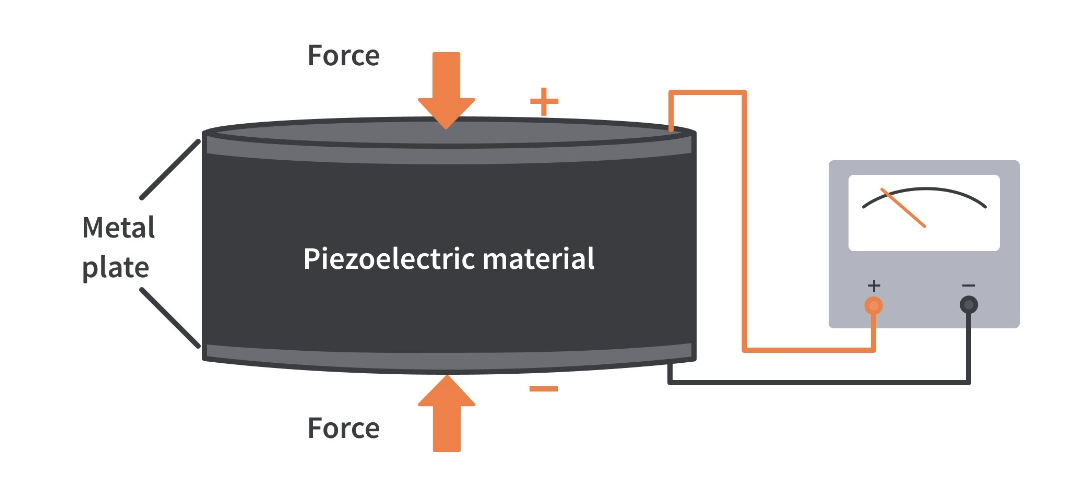
\includegraphics[width=0.7\textwidth]{Fundamentals/Piezoelectric-effect}
    \caption{Analog Piezoelectric Ceramic Vibration Module \cite{PiezoEffect}}
    \label{fig:PiezoEffect}
\end{figure}

%%%%%%%%%%%%%%%%%%%%%%%%%%%%%%%%%%%%%%%%%%%%%%%%%%%%%%%%%%%%%%%%%%%%%%%%%%%%%%%
\subsection{Piezoelectric ceramic vibration sensor}
\label{sec:PiezoelectricCeramicVibrationSensor}
Positive piezoelectric effect is the fundamental working mechanism of piezoelectric ceramic sensors. 
It is primarily used to measure physical quantities including acceleration, pressure, and vibration, as well as their fluctuations. 
As depicted in the figure \Ref*{fig:PiezoSensor}, a piezoelectric ceramic chip composed of lead zirconate titanate (PZT) is glued to a 
circular copper plate to create a piezoelectric ceramic element.

\begin{figure}[htbp]
    \centering
    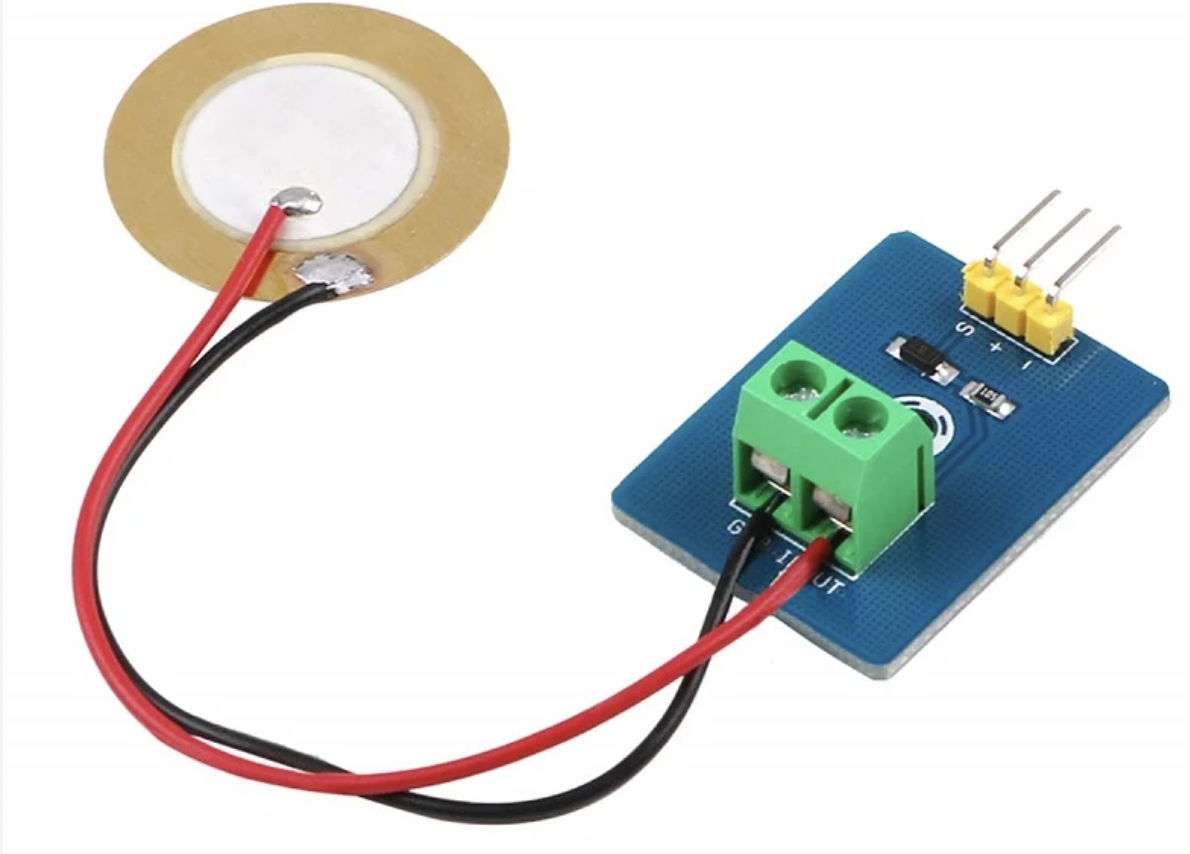
\includegraphics[width=0.6\textwidth]{Fundamentals/Piezo-ceramic-sensors}
    \caption{Analog Piezoelectric Ceramic Vibration Module \cite{PiezoSensor}}
    \label{fig:PiezoSensor}
\end{figure}

When the external high frequency vibration is felt (i.e., the external force varies periodically), 
the charge on the surface of the piezoelectric sensitive element also varies periodically, 
and the frequency of the change corresponds to that of the vibration. Collecting and measuring the charge signal 
on the surface of the piezoelectric sensitive element allows for the measurement of vibration. 
Its attributes include small size, quick frequency response, lack of an external power source, lack of heat, 
lack of noise, and high sensitivity.



%%%%%%%%%%%%%%%%%%%%%%%%%%%%%%%%%%%%%%%%%%%%%%%%%%%%%%%%%%%%%%%%%%%%%%%%%%%%%%%
                      %%   %%
%%%%%%%%%%%%%%%%%%%%%%%%%%%%%%%%%%%%%%%%%%%%%%%%%%%%%%%%%%%%%%%%%%%%%%%%%%%%%%%




%%%%%%%%%%%%%%%%%%%%%%%%%%%%%%%%%%%%%%%%%%%%%%%%%%%%%%%%%%%%%%%%%%%%%%%%%%%%%%%
                      %%Machine lerning%%
%%%%%%%%%%%%%%%%%%%%%%%%%%%%%%%%%%%%%%%%%%%%%%%%%%%%%%%%%%%%%%%%%%%%%%%%%%%%%%%